% ==============================================================================
% Appendix: Supplementary Figures and Tables
% ==============================================================================

\section{Supplementary Figures and Tables}
\label{app:figures}

\begin{figure}[ht]
  \centering
  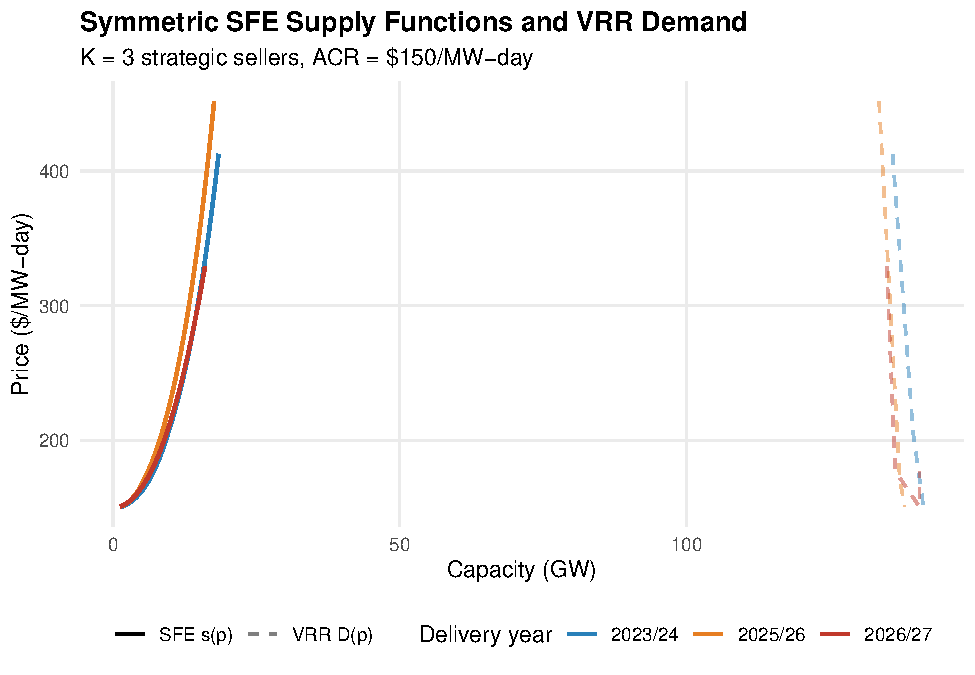
\includegraphics[width=0.85\textwidth]{../Figures/fig01_supply_functions.pdf}
  \caption{New VRR Design Compresses Equilibrium Supply Toward the Price Cap}
  \label{fig:supply_functions}
  {\small\noindent\textit{Notes:} Solid lines: equilibrium supply functions;
    dashed lines: VRR demand curves. Source: SFE model calibrated to PJM
    planning parameters, $K = 3$, $c = \$150$/MW-day.}
\end{figure}

\begin{table}[ht]
  \centering
  \caption{Equilibrium Price and Price-Cost Margin by $K$ (Baseline Calibration)}
  \label{tab:K_sensitivity}
  \begin{tabular}{lccc|ccc|ccc}
    \toprule
    & \multicolumn{3}{c|}{2023/24 (Old VRR)} &
      \multicolumn{3}{c|}{2025/26 (Old VRR)} &
      \multicolumn{3}{c}{2026/27 (New VRR)} \\
    $K$ & $p^*$ & $L$ & cap & $p^*$ & $L$ & cap & $p^*$ & $L$ & cap \\
    \midrule
    2  & 412 & 0.64 & \checkmark & 452 & 0.67 & \checkmark & 329 & 0.54 & \checkmark \\
    3  & 330 & 0.55 &            & 426 & 0.65 &            & 329 & 0.54 & \checkmark \\
    4  & 215 & 0.30 &            & 261 & 0.42 &            & 228 & 0.34 & \\
    5  & 168 & 0.11 &            & 184 & 0.19 &            & 177 & 0.15 & \\
    7  & 151 & 0.01 &            & 152 & 0.01 &            & 152 & 0.01 & \\
    10 & 151 & 0.01 &            & 151 & 0.01 &            & 151 & 0.01 & \\
    \bottomrule
  \end{tabular}
  \vspace{3pt}

  \begin{minipage}{0.92\textwidth}
    \footnotesize \textit{Notes:} Prices in \$/MW-day. $L = (p^* - c)/p^*$;
    $c = \$150$/MW-day. \checkmark\ indicates the market clears at the VRR
    price cap $\bar{p}$. Underlies Figure~\ref{fig:K_lerner} in
    Section~\ref{sec:results}.
  \end{minipage}
\end{table}

\begin{figure}[ht]
  \centering
  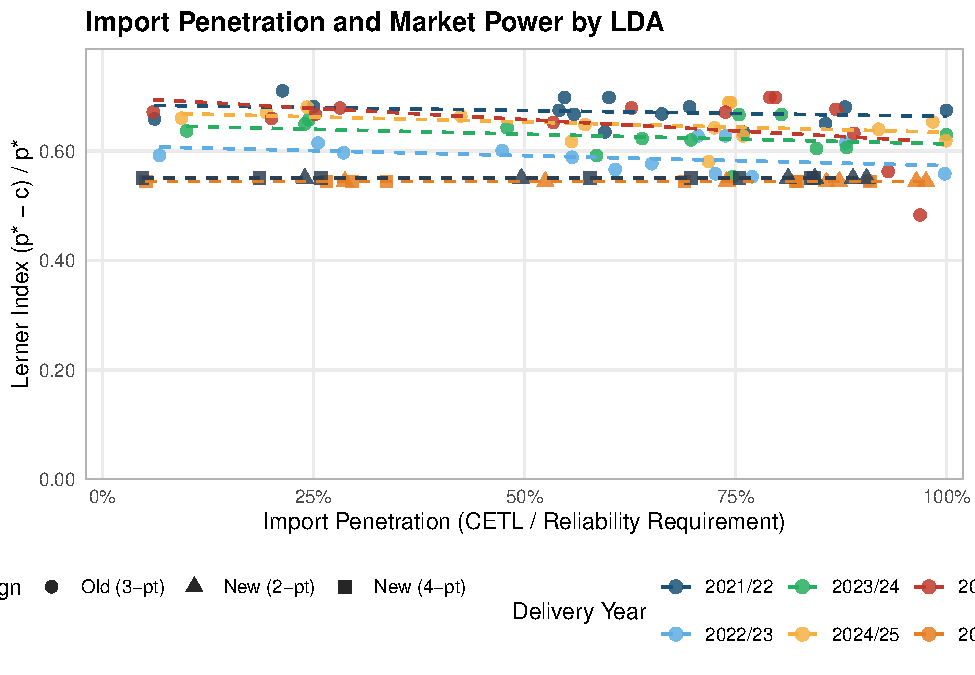
\includegraphics[width=0.85\textwidth]{../Figures/fig06_cetl_scatter.pdf}
  \caption{Higher Import Penetration Systematically Reduces Local Markups}
  \label{fig:cetl_scatter}
  {\small\noindent\textit{Notes:} Source: SFE model calibrated to PJM planning
    parameters and CETL data by LDA. Each point is one LDA-year observation;
    dashed lines are ordinary least squares (OLS) trends by year. Underlies
    the import-penetration claim in Section~\ref{subsec:res_lda}.}
\end{figure}
